% =====================================================================
% Castalia -- short overview deck.  Figures, schematics and spec tables;
% as few words as the slides can carry.
%
% Template: the ECEN 222 lecture deck (Berkeley theme, beaver colours,
% 16:9), see preamble.tex.
%
% Every plot, schematic and generated diagram is \input DIRECTLY from the
% shared TRM sources (implementations/asic/castalia/analog/ and the
% generated platform/common/latex/TRM/include/), so a regenerated TRM
% updates this deck.  The machinery is in trmreuse.tex; the only deck-local
% artwork is fig_marker_fusion.tex (clinical data the TRM carries as prose).
%
% Numbers on the spec slides are copied from the TRM build of 2026-09-15
% (Build 0155aecd) and the tapeout_review campaign record; each slide's
% source is named in a comment above it.
%
% Build:  make        (two pdflatex passes; copies the PDF next to TRM.pdf)
% =====================================================================
\documentclass[10pt, aspectratio=169]{beamer}

% =====================================================================
% preamble.tex -- lifted from the ECEN 222 lecture template
% (work/courses/instructor/ECEN222/latek/lectures/lecture08_opamps) via
% docs/publications/castalia_lab_talk, so this deck matches the course slides.  Berkeley theme, beaver colours,
% 16:9, custom two-box footline.  Additions for this deck are marked.
% =====================================================================
\usefonttheme{professionalfonts}

\mode<presentation>
{
  \usetheme{Berkeley}
  \usecolortheme{beaver}
  \usefonttheme{default}
  \setbeamertemplate{navigation symbols}{}
  \setbeamertemplate{caption}[numbered]
}

\setbeamertemplate{footline}{%
  \leavevmode%
  \hbox{%
    \begin{beamercolorbox}[wd=.85\paperwidth,ht=2.5ex,dp=1ex,left]{author in head/foot}%
      \usebeamerfont{author in head/foot}Maxx Seminario, Castalia overview%
    \end{beamercolorbox}%
    \begin{beamercolorbox}[wd=.15\paperwidth,ht=2.5ex,dp=1ex,right]{date in head/foot}%
      \hspace*{0.5em}\insertframenumber{} / \inserttotalframenumber\hspace*{0.5em}%
    \end{beamercolorbox}%
  }%
  \vskip0pt%
}

\usepackage[english]{babel}
\usepackage[utf8]{inputenc}
\usepackage{tikz}
\usetikzlibrary{shapes.geometric}
\usepackage{pgfplots}
\usepackage{array}
\usepackage{makecell}
\usepackage{verbatim}
\usepackage{graphicx}
\usepackage{subcaption}
\usepackage{amsfonts}
\usepackage{amsmath}
\usepackage{bm}
\usepackage{circuitikz}
\usepackage{caption}
\captionsetup{compatibility=false}
\usepackage[absolute,overlay]{textpos}
\usetikzlibrary{calc}
\usetikzlibrary{pgfplots.fillbetween, backgrounds}
\usetikzlibrary{positioning}
\usetikzlibrary{pgfplots.groupplots}
\usetikzlibrary{plotmarks}
\usepgfplotslibrary{groupplots}
\pgfplotsset{compat=newest}

% --- added for this deck ---------------------------------------------
\usepackage{booktabs}                 % the TRM's tables are booktabs
\usepackage{siunitx}                  % ... and its numbers are siunitx
\usepackage{placeins}                 % \FloatBarrier, used by TRM masters
\usepackage{bytefield}                % AddressSpaceDiagram
\usepackage{tikz-timing}              % the arbiter / mutex / IRQ waveform diagrams
\usepackage{tikzducks}                % placeholders for artwork not yet drawn
\usetikzlibrary{arrows.meta, fit, patterns, decorations.pathreplacing,
                decorations.markings, shapes.misc, matrix, chains}
\usepgfplotslibrary{statistics}
\usepackage{multirow}
\usepackage{colortbl}
\sisetup{detect-weight=true, detect-family=true}

% --- sidebar: dark, for readability -----------------------------------
% Berkeley's sidebar is a light tint by default and the section names in it
% wash out on a projector.  Dark ground with white type instead; the hue is
% the theme's own BeaverRed so it still reads as the ECEN 222 deck.
\definecolor{SidebarDark}{RGB}{72,18,18}
\setbeamercolor{sidebar}{bg=SidebarDark}
\setbeamercolor{palette sidebar primary}{fg=white}
\setbeamercolor{palette sidebar secondary}{fg=white!78}
\setbeamercolor{palette sidebar tertiary}{fg=white!78}
\setbeamercolor{palette sidebar quaternary}{fg=white}
\setbeamercolor{title in sidebar}{fg=white}
\setbeamercolor{author in sidebar}{fg=white!80}
\setbeamercolor{section in sidebar}{fg=white}
\setbeamercolor{section in sidebar shaded}{fg=white!55}
\setbeamercolor{subsection in sidebar}{fg=white!88}
\setbeamercolor{subsection in sidebar shaded}{fg=white!50}
\setbeamerfont{section in sidebar}{size=\tiny}
\setbeamerfont{section in sidebar shaded}{size=\tiny}

\usepackage{hyperref}
\definecolor{BeaverRed}{RGB}{179,38,38}
\hypersetup{
    colorlinks=true,
    linkcolor=BeaverRed,
    filecolor=magenta,
    urlcolor=cyan,
    % PDF metadata: this is the name the viewer's title bar and the file
    % properties show, and it is NOT taken from \title once set here.
    pdftitle={Castalia: a four-channel electrochemical sensing SoC},
    pdfauthor={Maxx A. Seminario},
    pdfsubject={Short overview deck, University of Nebraska-Lincoln},
    pdfkeywords={Castalia, VestaRV, RISC-V, potentiostat, electrochemical
                 sensing, ovarian cancer panel, 65 nm CMOS},
}

% Colored icons in itemize labels (ECEN 222 template, 01/06/2026)
\usepackage{wasysym}
\newcommand{\neutralface}{%
  \tikz[baseline=-0.6ex]{
    \draw (0,0) circle (0.9ex);
    \fill (-0.35ex,0.25ex) circle (0.12ex);
    \fill ( 0.35ex,0.25ex) circle (0.12ex);
    \draw (-0.35ex,-0.25ex) -- (0.35ex,-0.25ex);
  }%
}
\newcommand{\baditem}{\textcolor{red!70!black}{\frownie}}
\newcommand{\gooditem}{\textcolor{green!60!black}{\smiley}}
\newcommand{\mehitem}{\textcolor{orange!80!black}{\neutralface}}

% --- deck-local conveniences ------------------------------------------
% Slides in this deck carry very little text, so the default itemize
% spacing is loosened and the body font is set once here.
\setbeamertemplate{itemize items}[circle]
\setbeamerfont{itemize/enumerate body}{size=\small}
\setbeamerfont{itemize/enumerate subbody}{size=\footnotesize}
\setlength{\leftmargini}{1.2em}

% A "so what" strip: one line under a figure, in the accent colour.
\newcommand{\sowhat}[1]{\vfill{\scriptsize\color{BeaverRed}\textbf{#1}}\vspace{-0.1cm}}

% "New since the Myshkin tapeout" badge.  A lot of this deck is answering
% that question, so the answer is marked on the slide rather than said.
\newcommand{\newin}{{\scriptsize\color{BeaverRed}\textbf{[new since Myshkin]}}}

% Silicon / schematic provenance badges.  Every analog number in this deck
% is simulated; every digital number is from the hardened flow.  Saying so
% once per slide is cheaper than saying it once per number.
\newcommand{\badge}[2]{\textcolor{#1}{\footnotesize\ensuremath{\blacksquare}}\,{\scriptsize #2}}
\newcommand{\bsim}{\badge{orange!85!black}{schematic sim, pre-layout}}
\newcommand{\bext}{\badge{blue!70!black}{extracted netlist}}
\newcommand{\bflow}{\badge{green!45!black}{hardened flow, post-route}}
\newcommand{\bmc}{\badge{red!70!black}{Monte Carlo, 200 samples}}

% =====================================================================
% trmreuse.tex -- machinery for re-using Castalia TRM LaTeX fragments
% inside this Beamer deck, unmodified and un-copied.
% Originally written for docs/publications/castalia_lab_talk; this copy
% differs only in the path block below (relative, repo-anchored).
%
% The TRM's figure fragments (pgfplots plots, circuitikz schematics,
% generated TikZ block diagrams and booktabs tables) are \input directly
% from the TRM source tree, so a regenerated TRM updates this deck.  Two
% things have to be arranged for that to work:
%
%   1. path + macro context -- the fragments assume the TRM's cwd and a
%      handful of the TRM's own \newcommands.  Both are supplied below.
%   2. float suppression + captions -- a TRM caption is 3-5 sentences of
%      body text and belongs on a page, not a slide.  \trmfig strips the
%      float wrapper, the caption and the label, and scales what is left.
% =====================================================================

% --- where the shared sources live --------------------------------------
% This deck sits in implementations/asic/castalia/docs/deck/, next to the
% published TRM.pdf, and every path below is RELATIVE to that directory, so
% the deck moves with the repository.
%
%   \AnalogSrc  implementations/asic/castalia/analog/   the hand-written analog
%               chapter and the maestro2tex fig_/tab_/sch_ fragments -- the
%               tracked source that LatexUserGuide.CopyAnalogChapter copies
%               into the TRM build.  Read from the source, not the copy.
%   \TRMinc     platform/common/latex/TRM/include/      the GENERATED system
%               diagrams and defines.tex.  Gitignored; run `make generate`
%               (or `make chip`) in platform/common first.
%   \Assets     assets/web/                             the layout renders.
%   \ISCASroot  the ISCAS'27 paper (outside the repo) -- the concept figure
%               only, guarded with \IfFileExists so the deck builds without it.
\newcommand{\VestaRoot}{../../../../../}
\newcommand{\AnalogSrc}{../../analog/}
\newcommand{\TRMroot}{\VestaRoot platform/common/latex/TRM/}
\newcommand{\TRMinc}{\TRMroot include/}
\newcommand{\Assets}{\VestaRoot assets/web/}
\providecommand{\MaestroRoot}{\AnalogSrc}
\newcommand{\ISCASroot}{/home/mseminario2/work/ieee/ISCAS27/latek/}
\makeatletter\edef\input@path{{\TRMroot}{\TRMinc}{\AnalogSrc}{\ISCASroot}}\makeatother
\graphicspath{{\Assets}{\TRMroot figures/}{\ISCASroot Figures/}}
\pgfplotsset{table/search path={\ISCASroot}}

% --- the TRM macros the fragments use --------------------------------
% Verbatim from platform/common/latex/packages-commands.tex (all of them
% are plain \texttt wrappers) plus the generated defines.
\providecommand{\pin}[1]{\texttt{#1}}
\providecommand{\peripheral}[1]{\texttt{#1}}
\providecommand{\register}[1]{\texttt{#1}}
\providecommand{\bitfield}[1]{\texttt{#1}}
\providecommand{\asminline}[1]{\texttt{#1}}
\providecommand{\cinline}[1]{\texttt{#1}}
\providecommand{\forthinline}[1]{\texttt{#1}}
\providecommand{\bashinline}[1]{\texttt{#1}}
\input{\TRMinc defines.tex}

% \memsection -- structural, not a stub: AddressSpaceDiagram needs the real
% one.  Verbatim from platform/common/latex/packages-commands.tex line 93.
\providecommand{\memsection}[4]{%
	\bytefieldsetup{bitheight=#3\baselineskip}%
	\bitbox[]{10}{%
		\texttt{#1}
		\\
		\vspace{#3\baselineskip}
		\vspace{-2\baselineskip}
		\vspace{-#3pt}
		\texttt{#2}
	}%
	\bitbox{16}{#4}%
}

% --- the TRM figure theme (v* styles) --------------------------------
% Verbatim from platform/common/latex/packages-commands.template.tex: the
% generated diagrams (PowerDomainDiagram, ...) draw with these.
\definecolor{vestaRed}{rgb}{0.75,0,0}
\definecolor{vestaRedText}{rgb}{0.70,0,0}
\definecolor{vestaInk}{rgb}{0,0,0}
\tikzset{
	% Boxes. Three weights of fill, one stroke, one corner radius. The block
	% diagrams draw with vbox: a white box with the thin grey outline, the
	% RP2040 datasheet look; the filled weights stay defined for the figures
	% that tell two kinds of node apart by weight.
	vbox/.style={line width=0.6pt, rounded corners=2pt, draw=black!70, fill=white},
	vblock/.style={thick, rounded corners=2pt, draw=vestaInk, fill=black!8},
	vblocklt/.style={thick, rounded corners=2pt, draw=vestaInk, fill=black!3},
	vblockw/.style={thick, rounded corners=2pt, draw=vestaInk, fill=white},
	vblockem/.style={line width=1.1pt, rounded corners=2pt, draw=vestaInk, fill=black!12},
	% The bus bar, and the package boundary.
	vbar/.style={thick, draw=vestaInk, fill=black!15},
	vbound/.style={draw=vestaRed, line width=1.2pt},
	% A grouping region: a thin dashed outline that leaves the paper white, never a
	% full-bleed grey band.
	vregion/.style={draw=black!35, line width=0.5pt, dashed, rounded corners=3pt},
	% Text: sans throughout, in two sizes only. vname (\small) names a block, vlab
	% (\footnotesize) carries everything secondary, and nothing is set below
	% \footnotesize, so the smallest label is 8 pt at natural size. The older names
	% stay defined, at the same floor, for the emitters that still use them.
	vname/.style={font=\sffamily\small, align=center, inner sep=1pt},
	vlab/.style={font=\sffamily\footnotesize, align=center, inner sep=1pt},
	vhd/.style={font=\sffamily\footnotesize, align=center, inner sep=1pt, anchor=north},
	vbc/.style={font=\sffamily\footnotesize, align=center, inner sep=1pt},
	vsm/.style={font=\sffamily\footnotesize, align=center, inner sep=1pt},
	vnote/.style={font=\sffamily\footnotesize\itshape, text=black!55, align=left, inner sep=1.5pt},
	vgroup/.style={font=\sffamily\small\itshape, text=black!55, align=left, fill=white, inner sep=1.5pt},
	vredlab/.style={font=\sffamily\small\bfseries, text=vestaRedText, align=left},
	% Lines: one arrow head for the whole manual, Stealth, on every style that carries
	% a head, and a junction dot where a wire really joins another.
	vwire/.style={semithick, draw=vestaInk},
	vflow/.style={->, >={Stealth[length=2mm]}, semithick, draw=vestaInk},
	vbus/.style={<->, >={Stealth[length=2mm]}, thick, draw=vestaInk},
	vaccent/.style={->, >={Stealth[length=2mm]}, semithick, draw=vestaRed},
	vghost/.style={dashed, draw=black!45, semithick},
	vdot/.style={circle, fill=vestaInk, inner sep=0pt, minimum size=3pt},
	% A mux: a trapezium standing on its narrow side, inputs on the wide (left) edge,
	% the select code beside each input.
	vmux/.style={trapezium, trapezium angle=70, shape border rotate=270, line width=0.6pt, draw=black!70, fill=white, inner sep=1pt},
}

% --- schematics: heavier strokes for projection ------------------------
% The TRM's circuitikz schematics are drawn for print at 0.4-0.6 pt.  On a
% slide they vanish, so every path inside a \trmfit'd fragment is drawn one
% step heavier; explicit "thick" rails stay relatively heavier still.
\newcommand{\trmslidestrokes}{%
  \tikzset{every path/.append style={line width=0.9pt}}%
  \ctikzset{bipoles/thickness=1.3}%
}

% \memrow / \memgap -- the address-column rows AddressSpaceDiagram uses since
% the 2026-09 TRM (verbatim from packages-commands.template.tex).
\providecommand{\memrow}[3]{%
	\bytefieldsetup{bitheight=#2\baselineskip}%
	\bitbox[]{10}{%
		\texttt{#1}
		\\
		\vspace{#2\baselineskip}
		\vspace{-2\baselineskip}
		\vspace{-#2pt}
		\mbox{}
	}%
	\bitbox{16}{\sffamily\small #3}%
}
\providecommand{\memgap}[2]{%
	\bytefieldsetup{bitheight=#2\baselineskip}%
	\bitbox[]{10}{%
		\texttt{#1}
		\\
		\vspace{#2\baselineskip}
		\vspace{-2\baselineskip}
		\vspace{-#2pt}
		\mbox{}
	}%
	\bitbox{16}[bgcolor=black!8]{}%
}

% --- the maestro2tex categorical palette -----------------------------
% Slots 1-5 of the validated reference palette, in documented order; the
% block masters declare these with \providecolor, individual fig_*.tex do not.
\definecolor{mtxA}{HTML}{2A78D6}
\definecolor{mtxB}{HTML}{EB6834}
\definecolor{mtxC}{HTML}{1BAF7A}
\definecolor{mtxD}{HTML}{EDA100}
\definecolor{mtxE}{HTML}{E87BA4}

% --- \trmfig[scale]{fragment.tex} ------------------------------------
% Inputs a TRM fragment with its float, caption and label removed and the
% result scaled.  Everything is done inside a group so the redefinitions
% never escape onto the rest of the slide.
\newsavebox{\trmbox}
\newcommand{\trmfig}[2][0.62]{%
  \begingroup
    \renewenvironment{figure}[1][]{\ignorespaces}{}%
    \renewenvironment{table}[1][]{\ignorespaces}{}%
    \renewcommand{\caption}[2][]{}%
    \renewcommand{\label}[1]{}%
    \renewcommand{\FloatBarrier}{}%
    \sbox{\trmbox}{\begin{minipage}{\linewidth}\centering\input{#2}\end{minipage}}%
    \scalebox{#1}{\usebox{\trmbox}}%
  \endgroup}

% \trmtab -- same, for a booktabs table fragment (no scaling by default).
\newcommand{\trmtab}[2][1.0]{\trmfig[#1]{#2}}

% \trmfigw[width fraction]{fragment.tex} -- same, but fitted to a fraction
% of \linewidth instead of scaled by a factor.  Use this for the wide
% generated block diagrams, whose natural width is 20-34 cm.
\newcommand{\trmfigw}[2][1.0]{%
  \begingroup
    \renewenvironment{figure}[1][]{\ignorespaces}{}%
    \renewenvironment{table}[1][]{\ignorespaces}{}%
    \renewcommand{\caption}[2][]{}%
    \renewcommand{\label}[1]{}%
    \renewcommand{\FloatBarrier}{}%
    \sbox{\trmbox}{\input{#2}}%
    \resizebox{#1\linewidth}{!}{\usebox{\trmbox}}%
  \endgroup}

% \trmfigh{height}{fragment.tex} -- fitted to a stated height.  The usable
% body height of a 16:9 Berkeley frame is about 6.6 cm.
\newcommand{\trmfigh}[2]{%
  \begingroup
    \renewenvironment{figure}[1][]{\ignorespaces}{}%
    \renewenvironment{table}[1][]{\ignorespaces}{}%
    \renewcommand{\caption}[2][]{}%
    \renewcommand{\label}[1]{}%
    \renewcommand{\FloatBarrier}{}%
    \sbox{\trmbox}{\input{#2}}%
    \resizebox*{!}{#1}{\usebox{\trmbox}}%
  \endgroup}

% =====================================================================
% \duckph{width}{what the missing artwork is}
% Placeholder for artwork that does not exist yet -- the top-level GDS
% plot, die photographs, bonding diagrams.  A tikzducks duck in a dashed
% frame: impossible to mistake for a real figure on a projector, and
% impossible to leave in by accident.
% =====================================================================
\newcommand{\duckph}[3][graduate, book, bookcolour=red!60!black]{%
  \begin{center}
  \setlength{\fboxsep}{6pt}%
  \tikz[baseline]{\node[draw=red!70!black, very thick, dashed, rounded corners=3pt,
        inner sep=8pt, align=center, text width=#2]{%
     {\bfseries\color{red!70!black} ARTWORK PENDING}\\[4pt]
     \begin{tikzpicture}[scale=0.95]
       \duck[#1]
     \end{tikzpicture}\\[4pt]
     {\small #3}};}
  \end{center}}

% =====================================================================
% \trmfit[natural width]{max width}{max height}{fragment.tex}
%
% Fits a fragment inside a BOX, scaling uniformly by whichever limit binds
% first, so it can be dropped into a column without overflowing either way.
% This is the one to reach for by default.
%
% WHY THE OPTIONAL FIRST ARGUMENT MATTERS.  Every generated pgfplots
% fragment declares "width=0.82\linewidth, height=6.2cm" -- a RELATIVE
% width against an ABSOLUTE height.  Input inside a half-slide beamer
% column, \linewidth is about 5.9 cm, so the axis comes out 4.8 cm wide by
% 6.2 cm tall: portrait, and every trace squashed in x.  Scaling that box
% afterwards cannot undo it -- the aspect is already wrong.
%
% So \trmfit sets \hsize/\linewidth/\columnwidth to a wide value BEFORE the
% \input, which is what the fragment's 0.82\linewidth then resolves
% against.  The plot is laid out landscape and only then scaled down to
% fit.  15 cm gives roughly 12.3 x 6.2 cm, a 2:1 axis.  Pass a smaller
% value for a fragment that should come out squarer, larger for a wider one.
% Circuitikz fragments (which use \resizebox{\linewidth}{!}) are unaffected:
% they are laid out at the natural width and scaled back uniformly.
% =====================================================================
\newlength{\trmnat}
\newcommand{\trmfit}[4][15cm]{%
  \begingroup
    \renewenvironment{figure}[1][]{\ignorespaces}{}%
    \renewenvironment{table}[1][]{\ignorespaces}{}%
    \renewcommand{\caption}[2][]{}%
    \renewcommand{\label}[1]{}%
    \renewcommand{\FloatBarrier}{}%
    \setlength{\trmnat}{#1}%
    % \linewidth is set as a VALUE for the fragment to resolve against, but
    % the box is NOT wrapped in a minipage of that width -- a minipage would
    % pin \wd\trmbox to \trmnat and the fit below would then scale a 33 cm
    % TikZ diagram as though it were 15 cm wide, and it would run off the slide.
    \sbox{\trmbox}{\hsize=\trmnat \linewidth=\trmnat \columnwidth=\trmnat
                   \trmslidestrokes\input{#4}}%
    % natural TOTAL height (ht+dp: a tabular is centred on the baseline, so dp
    % is half of it), then the height the box would have if scaled to width #2
    \dimen0=\ht\trmbox \advance\dimen0 by \dp\trmbox
    \divide\dimen0 by 64                      % keep the product inside 2^31 sp
    \count0=\wd\trmbox  \divide\count0 by 65536
    \count2=\dimexpr#2\relax \divide\count2 by 65536
    \ifnum\count0<1 \count0=1 \fi
    \multiply\dimen0 by \count2
    \divide\dimen0 by \count0
    \multiply\dimen0 by 64
    \ifdim\dimen0>\dimexpr#3\relax
      \resizebox*{!}{#3}{\usebox{\trmbox}}%    height binds (starred: TOTAL height,
                                               % a tabular sits centred on the baseline)
    \else
      \resizebox{#2}{!}{\usebox{\trmbox}}%     width binds
    \fi
  \endgroup}


\title[Castalia]{Castalia}
\subtitle{A four-channel electrochemical sensing SoC with a five-hart RISC-V back end}
\author{Maxx Seminario}
\institute{University of Nebraska--Lincoln}
\date{\today}

\begin{document}

\begin{frame}
  \titlepage
\end{frame}

% =====================================================================
\section{Target application}

% Source: ISCAS'27 draft, Fig. 1 candidate B (outside the repo; guarded).
\begin{frame}{One serum aliquot, four sites, one score}
\IfFileExists{\ISCASroot Figures/concept_cand_B.tex}{%
  \centering\resizebox{!}{5.6cm}{\input{\ISCASroot Figures/concept_cand_B.tex}}%
}{%
  \duckph{9cm}{ISCAS'27 concept figure (\texttt{concept\_cand\_B.tex}) not found on this machine}%
}
\sowhat{Symptomatic-patient triage on a disposable four-site cartridge; four markers read at the same instant, fused on chip.}
\end{frame}

% Source: Chen et al. 2018 (458 patients), as carried in the ISCAS'27 introduction.
\begin{frame}{No single ovarian marker is a usable test}
\begin{columns}[T]
\column{0.64\textwidth}
\vspace{0.1cm}
\resizebox{\linewidth}{!}{%% HAND-DRAWN for this deck, from the ISCAS'27 introduction.
%%
%% Chen et al. 2018, four markers measured individually on the same 458
%% patients, then fused.  Individually none of them is a usable test; the
%% combination is.  This is the slide that answers "why four channels":
%% the clinically useful decision is a learned combination of markers, so
%% the natural unit of integration is four concurrent channels plus the
%% processor that combines them, not one better potentiostat.

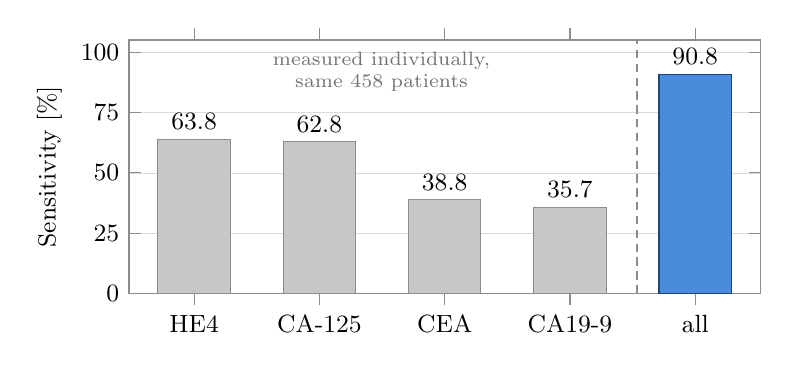
\begin{tikzpicture}
  \begin{axis}[
    width=9.6cm, height=4.8cm,
    ybar, bar width=0.92cm,
    ymin=0, ymax=105,
    ylabel={Sensitivity [\%]},
    symbolic x coords={HE4, CA-125, CEA, CA19-9, fused},
    % explicit: xtick=data would take the FIRST plot's coordinates only
    xtick={HE4, CA-125, CEA, CA19-9, fused},
    xticklabels={HE4, CA-125, CEA, CA19-9, all},
    xticklabel style={font=\small, align=center},
    ylabel style={font=\small},
    yticklabel style={font=\small},
    ytick={0,25,50,75,100},
    grid=major, ymajorgrids=true, xmajorgrids=false,
    major grid style={line width=0.2pt, draw=black!14},
    axis line style={line width=0.4pt, draw=black!45},
    tick style={line width=0.4pt, draw=black!45},
    enlarge x limits=0.13,
    nodes near coords, nodes near coords style={font=\small\bfseries},
    every node near coord/.append style={/pgf/number format/fixed,
                                         /pgf/number format/precision=1},
  ]
    % bar shift=0pt: two \addplots under ybar are otherwise offset side by
    % side, which puts every bar off its tick.
    \addplot[draw=black!45, fill=black!22, bar shift=0pt] coordinates
      {(HE4,63.8) (CA-125,62.8) (CEA,38.8) (CA19-9,35.7)};
    \addplot[draw=mtxA!60!black, fill=mtxA!85, bar shift=0pt] coordinates {(fused,90.8)};
    % annotations in axis-relative coordinates, so they follow the axis box
    \draw[black!45, densely dashed, line width=0.6pt]
      (rel axis cs:0.805,0) -- (rel axis cs:0.805,1);
    \node[font=\scriptsize, black!55, anchor=north, align=center]
      at (rel axis cs:0.40,0.99) {measured individually,\\ same 458 patients};
  \end{axis}
\end{tikzpicture}
}
\column{0.34\textwidth}
\vspace{0.6cm}
{\footnotesize
\begin{tabular}{@{}lr@{}}
\toprule
Panel & Sensitivity \\
\midrule
Best single (HE4)  & 63.8\,\% \\
Four fused         & \textbf{90.8\,\%} \\
\midrule
ROMA, FDA-cleared  & 2 markers \\
This chip          & 4 channels \\
\bottomrule
\end{tabular}}
\end{columns}
\sowhat{Clinical data, not simulation. The decision is a learned combination, so the unit of integration is four concurrent channels plus the processor that fuses them.}
\end{frame}

% Source: TRM fig_electrode_dpv (analog/), schematic-level channel.
\begin{frame}{Four markers resolved in one differential-pulse sweep}
\centering\trmfit{\linewidth}{5.6cm}{\MaestroRoot fig_electrode_dpv.tex}
\vspace{0.05cm}
{\centering\bsim\par}
\sowhat{Peak position identifies the reporter, peak height carries concentration. Apexes within 2\,mV and 1\,\% of the assay targets; blank below 1\,pA.}
\end{frame}

% Source: TRM fig_electrode_dose (analog/).
\begin{frame}{Every clinical cut-off lands inside the channel window}
\centering\trmfit{\linewidth}{5.6cm}{\MaestroRoot fig_electrode_dose.tex}
\vspace{0.05cm}
{\centering\bsim\par}
\sowhat{CA-125 35\,U/mL, HE4 70\,pmol/L, CA19-9 37\,U/mL, CEA 5\,ng/mL: all four on the steep part of the curve at one $R_f$ setting.}
\end{frame}

% =====================================================================
\section{The chip}

% Sources: TRM 2.1 Features and Fig. 2.1 (2026-09-15); tapeout_review/PLAN.md
% for die, package, pads and power.  Analog rows: TRM Ch. 33.
\begin{frame}{Castalia at a glance}
\vspace{-0.1cm}
\begin{columns}[T]
\column{0.49\textwidth}
{\scriptsize
\begin{tabular}{@{}ll@{}}
\multicolumn{2}{@{}l}{\textbf{\normalsize Digital}}\\[2pt]
\toprule
Harts            & 5 (1 orchestrator, 4 channel tiles) \\
ISA              & \texttt{rv32imac\_zba\_zbb\_zbs\_zbc} \\
Clock            & 24\,MHz rated, closed at 25\,MHz \\
Measured CPI     & 1.260 aggregate, nine benchmarks \\
Private TCM      & 8\,KiB per hart, 1-cycle \\
Shared RAM       & 80\,KiB behind a round-robin arbiter \\
Synchronisation  & 16 hardware mutexes, LR/SC, AMOs \\
Interrupts       & claim/complete, any vector to any hart \\
Accelerator      & NPU: MLP, conv-1D, XNOR, GEMM \\
Power domains    & 4 MTCMOS, one per channel tile \\
Debug            & JTAG, RISC-V Debug Module \\
Field boot       & NFC ISO 14443A harvested boot \\
\bottomrule
\end{tabular}}
\column{0.49\textwidth}
{\scriptsize
\begin{tabular}{@{}ll@{}}
\multicolumn{2}{@{}l}{\textbf{\normalsize Analog and physical}}\\[2pt]
\toprule
Measurement sites  & 4 identical, simultaneous \\
Topology           & bipolar grounded-WE potentiostat \\
Electrode pads     & 12 (CE/RE/WE $\times$ 4) \\
Converter          & 10-bit SAR per channel, extracted \\
Reference DAC      & 12-bit R--2R per channel \\
Feedback resistor  & 18\,k$\Omega + 6$\,k$\Omega\cdot N$, 320 codes \\
Full scale         & $\pm$40.7\,\textmu A to $\pm$0.41\,\textmu A \\
EIS                & firmware mode of the same channels \\
Analog supply      & 2.5\,V, $v_\mathrm{cm} = 1.25$\,V \\
\midrule
Process            & 65\,nm CMOS, 1P8M, HVT cells \\
Die / package      & $3.0\times3.0$\,mm / LQFP-100 \\
Digital power      & 10.72\,mW post-route, SS, 25\,MHz \\
\bottomrule
\end{tabular}}
\end{columns}
\sowhat{Digital numbers from the hardened flow; analog numbers schematic-level, except the SAR, which is extracted.}
\end{frame}

% Source: the ISCAS'27 paper's block diagram, drawn for a reader (outside
% the repo; guarded).  Fallback: the TRM's generated ChipSystemDiagram, which
% regenerates with the chip configuration but is too dense for a slide.
% The paper PNG predates the September configuration (it shows a 16 KiB boot
% ROM, SPI x2, I2C x2 against the TRM's 8 KiB, x3, x4); the topology is the same.
\begin{frame}{Block diagram}
\IfFileExists{\ISCASroot Figures/castalia_block_diagram.png}{%
  \centering
\includegraphics[width=\linewidth]{castalia_block_diagram.png}%
}{%
  \centering\trmfit[20cm]{\linewidth}{6.0cm}{\TRMinc ChipSystemDiagram.tex}%
}
\sowhat{Four channel tiles own four AFE sites; every master reaches ROM, RAM, NPU and peripherals only through the arbiter.}
\end{frame}

% Sources: assets/web renders (2026-07 signoff GDS); tapeout_review/PLAN.md
% for die and core box; TRM Ch. 3 for the package.
\begin{frame}{Physical implementation}
\begin{columns}[T]
\column{0.34\textwidth}
\centering

\includegraphics[width=\linewidth]{layout_castalia_chip_top.png}\\[2pt]
{\tiny chip top, $3.0\times3.0$\,mm}
\column{0.24\textwidth}
\centering

\includegraphics[width=\linewidth]{layout_hart_tile.png}\\[2pt]
{\tiny one hardened channel tile}
\column{0.40\textwidth}
\vspace{0.3cm}
{\footnotesize
\begin{tabular}{@{}ll@{}}
\toprule
Process    & 65\,nm, 1P8M, HVT \\
Core box   & $2690\times2690$\,\textmu m \\
Tile       & $660\times880$\,\textmu m \\
Tile logic & $\approx$98\,k NAND2-eq. \\
Tile SRAM  & 8\,KiB \\
Package    & LQFP-100, $14\times14$\,mm \\
\bottomrule
\end{tabular}}
\vspace{0.3cm}

\bflow
\end{columns}
\sowhat{One tile hardened once, instantiated four times; the notch in each tile is the analog channel's keep-out.}
\end{frame}

% Sources: post-route power report (SS 0.9 V 125 C, 25 MHz, activity 0.2);
% TRM Table 10.3 for CPI.
\begin{frame}{Digital, as closed}
\begin{columns}[T]
\column{0.30\textwidth}
\begin{block}{Whole chip, post-route}
\footnotesize
\begin{tabular}{@{}lr@{}}
\toprule
Internal   & 3.78\,mW \\
Switching  & 2.33\,mW \\
Leakage    & 4.61\,mW \\
\midrule
\textbf{Total} & \textbf{10.72\,mW} \\
\bottomrule
\end{tabular}
\end{block}
\begin{block}{One channel tile}
\footnotesize
\begin{tabular}{@{}lr@{}}
\toprule
Total      & 1.761\,mW \\
Gated      & 0 \\
\bottomrule
\end{tabular}
\end{block}
\column{0.36\textwidth}
\begin{block}{Measured CPI, timed kernels}
\scriptsize
\begin{tabular}{@{}lrr@{}}
\toprule
Benchmark & Instr. & CPI \\
\midrule
spmv      & 802\,447 & 1.143 \\
multiply  &  20\,892 & 1.163 \\
vvadd     &   2\,408 & 1.374 \\
median    &   4\,015 & 1.398 \\
qsort     & 123\,205 & 1.398 \\
rsort     & 146\,548 & 1.412 \\
dhrystone & 200\,523 & 1.504 \\
towers    &   3\,747 & 1.682 \\
memcpy    &  11\,017 & 1.726 \\
\midrule
\textbf{Aggregate} & \textbf{1\,314\,802} & \textbf{1.260} \\
\bottomrule
\end{tabular}
\end{block}
\column{0.30\textwidth}
\begin{block}{Timing at 25\,MHz}
\footnotesize
\begin{tabular}{@{}lr@{}}
\toprule
reg2reg WNS & $+$99\,ps \\
Leakage share & 43\,\% \\
\bottomrule
\end{tabular}
\end{block}
\vspace{0.2cm}
\bflow
\end{columns}
\sowhat{SS 0.9\,V 125\,\textdegree C, statistical activity 0.2. Gating one tile removes 1.76\,mW; the always-on band pays nothing.}
\end{frame}

% =====================================================================
\section{Analog front end}

% Source: TRM sch_tb_pixel (analog/).
\begin{frame}{Grounded-WE two-amplifier potentiostat}
\centering\trmfit[20cm]{\linewidth}{6.3cm}{\MaestroRoot sch_tb_pixel.tex}
\sowhat{A1 drives CE with RE in feedback; A2 holds WE at $v_\mathrm{cm}$ through $R_f$. $v_\mathrm{out} = v_\mathrm{cm} - I_\mathrm{we} R_f$, both polarities.}
\end{frame}

% Source: TRM fig_px_xover_ierr (analog/).
\begin{frame}{Bipolar accuracy through zero}
\centering\trmfit{\linewidth}{5.6cm}{\MaestroRoot fig_px_xover_ierr.tex}
\vspace{0.05cm}
{\centering\bsim\par}
\sowhat{No kink at the crossing: class-AB output, no dead zone. This is the measurement rev-1's PMOS mirror could not make.}
\end{frame}

% Source: TRM fig_pixtop_cv (analog/), assembled channel with its own DAC and SAR.
\begin{frame}{Cyclic voltammetry through the assembled channel}
\centering\trmfit{\linewidth}{5.6cm}{\MaestroRoot fig_pixtop_cv.tex}
\vspace{0.05cm}
{\centering\bsim\par}
\sowhat{Staircase potential from the on-chip DAC, current digitised by the on-chip SAR, unclipped over the sweep.}
\end{frame}

% Source: TRM fig_tiarprog_r_vs_code (analog/).
\begin{frame}{Programmable feedback resistor: one string, 320 codes}
\begin{columns}[T]
\column{0.64\textwidth}
\trmfit[13cm]{\linewidth}{5.6cm}{\MaestroRoot fig_tiarprog_r_vs_code.tex}
\column{0.34\textwidth}
\vspace{0.3cm}
\[ R_f = 18\,\mathrm{k}\Omega + 6\,\mathrm{k}\Omega\cdot N \]
{\footnotesize
\begin{tabular}{@{}lrr@{}}
\toprule
$N$ & $R_f$ & Full scale \\
\midrule
0   & 19.6\,k$\Omega$  & $\pm$40.7\,\textmu A \\
63  & 397\,k$\Omega$   & $\pm$2.02\,\textmu A \\
319 & 1.93\,M$\Omega$  & $\pm$0.41\,\textmu A \\
\midrule
LSB at 319 & \multicolumn{2}{r}{0.824\,nA} \\
\bottomrule
\end{tabular}}
\end{columns}
\sowhat{Strictly monotonic at every corner, including the four thermometer seams. Maximum gain is noise-limited, not quantisation-limited.}
\end{frame}

% Source: TRM fig_adc_transfer (analog/), extracted anatop_pixel_adc.
\begin{frame}{10-bit SAR ADC, extracted netlist}
\centering\trmfit{\linewidth}{5.4cm}{\MaestroRoot fig_adc_transfer.tex}
\vspace{0.05cm}
{\centering\bext\par}
\sowhat{23 clocks per conversion, 870\,kSa/s, 50\,pJ. The capacitor array exists only in layout, so this is the one block characterised extracted.}
\end{frame}

% Source: TRM fig_eis_error (analog/).
\begin{frame}{Impedance spectroscopy on the same channel}
\centering\trmfit[17cm]{\linewidth}{5.0cm}{\MaestroRoot fig_eis_error.tex}
\vspace{0.1cm}

{\footnotesize\centering
\resizebox{\linewidth}{!}{%
\begin{tabular}{@{}cccc@{}}
\toprule
Excitation & Demodulation & Accuracy & $|Z|$ range \\
\midrule
2-code DAC square & firmware, channel hart & $\pm$1\,\%, $\pm$0.6\textdegree{} to 5.05\,kHz; $\pm$5\,\% to 26.5\,kHz & 246\,$\Omega$ -- 12.1\,M$\Omega$ \\
\bottomrule
\end{tabular}}\par}
\vspace{0.05cm}
{\centering\bsim\par}
\sowhat{No EIS engine. Impedance is a ratio of two readings through one converter; the DAC drops out of the accuracy budget.}
\end{frame}

% Source: TRM Ch. 33 measurement tables (analog/note_meas_*.tex).
\begin{frame}{One AFE channel, as simulated}
\vspace{-0.05cm}
\centering
\resizebox{\linewidth}{!}{%
\begin{tabular}{@{}lll@{}}
\toprule
Parameter & Value & Condition \\
\midrule
CE compliance           & 13.2\,mV -- 2.480\,V          & 2.5\,V rail, corners \\
Cell current delivered  & $\pm$52.5\,\textmu A          & 12\,k$\Omega$ cell \\
TIA compliance          & $\pm$0.80\,V about $v_\mathrm{cm}$ & \\
Feedback resistor       & 19.6\,k$\Omega$ -- 1.93\,M$\Omega$, 320 codes & monotonic at every corner \\
Full-scale current      & $\pm$40.7\,\textmu A ($N{=}0$) to $\pm$0.41\,\textmu A ($N{=}319$) & SAR window $\cap$ TIA compliance \\
Current quantum         & 0.824\,nA at maximum gain     & below the 2\,nA noise budget \\
Bipolar accuracy        & 0.25--0.38 LSB worst          & 560\,k$\Omega$, 1\,M$\Omega$ electrode, corners \\
Control-loop PM         & 79--80\textdegree             & five corners, into a cell \\
TIA-loop PM             & 89--93\textdegree             & 12-cell electrode grid \\
Input current noise     & 341\,pA standalone, 3.6--21\,nA into an electrode & 0.1--100\,Hz, 560\,k$\Omega$ \\
Zero-current offset     & $\sigma(v_\mathrm{re}) = 5.72$\,mV, gain-independent & 200 MC samples, calibratable \\
Quiescent current       & 197--250\,\textmu A per channel & amplifiers $+$ local bias \\
\bottomrule
\end{tabular}}
\vspace{0.15cm}

{\centering\bsim\quad\bmc\par}
\sowhat{Pre-layout, electrode held nominal: no row includes electrode-to-electrode spread.}
\end{frame}

% =====================================================================
\section{From currents to a score}

% Source: TRM Ch. 17 (NPU), ISCAS'27 draft for the fusion form.
\begin{frame}{The fusion runs on the NPU}
\begin{columns}[T]
\column{0.50\textwidth}
\vspace{0.4cm}
\[ s = \sigma\Big(\sum_{k=1}^{4} w_k\,\hat{c}_k + b\Big) \]
\vspace{0.1cm}

{\footnotesize
\begin{tabular}{@{}ll@{}}
\toprule
Input  & peak current, peak potential, baseline $\times$ 4 \\
Mode   & 0, dense layer, one sigmoid \\
Output & one risk score \\
Weights & trained off-chip, staged by firmware \\
\bottomrule
\end{tabular}}
\column{0.46\textwidth}
\vspace{0.2cm}
{\footnotesize
\begin{tabular}{@{}ll@{}}
\toprule
\multicolumn{2}{@{}l}{\textbf{Per site}}\\
\midrule
Hart      & 1, ownership enforced in hardware \\
Potential & own 12-bit DAC \\
Converter & own 10-bit SAR \\
Power     & own MTCMOS domain \\
\bottomrule
\end{tabular}}
\end{columns}
\sowhat{The logistic form of the cleared two-marker algorithm, extended to four inputs and moved from the central laboratory onto the electrode.}
\end{frame}

\end{document}
